\documentclass[12pt]{article}
\usepackage{baseset}
\usepackage{myproblem}
\usepackage{stackengine}
\DeclareSymbolFont{operators}{OT1}{ntxtlf}{m}{n}
\SetSymbolFont{operators}{bold}{OT1}{ntxtlf}{b}{n}
\usepackage{wasysym}
\newcommand{\RomanNumeralCaps}[1]
{\MakeUppercase{\romannumeral #1}}
\usepackage{tabularx}
\usepackage{enumitem}

\begin{document}
\begin{tabularx}{\textwidth}{Xr}
{\Large \textbf{Астрофиз}} & Взлёт $3.11.2024$ \\
\end{tabularx}
\noindent\rule{\textwidth}{0.4pt}
\begin{enumerate}
    \item Определите, во сколько раз Сириуc ($-1.46^{m}$) ярче Ригеля ($0.12^m$).
    \item Экзопланета может быть обнаружена транзитным методом (изменение яркости звезды в моменты прохождения планеты по диску звезды), если диск планеты перекроет $1\%$ поверхности звезды. Определите, насколько изменяется звездная величина звезды в такие моменты?
    \item Двойная система состоит из звезд $5^{m}$ и $3^{m}$. Определите суммарную звездную величину двойной системы. 
    \item Тройная система состоит из звезд $3^{m}$, $4^{m}$  и $6^{m}$. Определите суммарную звездную величину тройной системы.
    \item Определите звездные величины компонент A и В звезды $\alpha$ Cen, если суммарная звездная величина -- $-0.27^m$, а соотношение светимостей компонент -- $3.47$.
    \item На рисунке приведена кривая блеска  затменно-переменной звезды. Определите по графику блеск компонентов двойной системы.

    \begin{figure}[h] 	
        \centering
        \begin{tikzpicture} 
        \begin{axis}[xlabel=время,
        ylabel=звездная величина, 
        grid=major, 
        y dir=reverse, 
        width=10cm, 
        legend pos = south west,
        ymax=3.2]
        \addplot[line width=1pt, black] coordinates {
            (0, 2)(1, 2)(1.9, 2.4)(2.1, 2.4)(3, 2)(4, 2)(4.9, 3.0)(5.1, 3.0)(6, 2)(7, 2)(7.9, 2.4)(8.1, 2.4)(9, 2)(10, 2)(10.9, 3.0)(11.1, 3.0)(12, 2)(13, 2)
        };
    
        \end{axis}
        \end{tikzpicture} 
    \end{figure} 
    \item Определите суммарную звездную величину шарового скопления с $10^{6}$ звезд звездной величины $19^m$.
    \item Шаровое скопление содержит $10^{6}$ звезд звездной величины $22^m$ и $10 000$ сверхгигантов со звездной величиной $17^m$. Сможем ли мы увидеть это шаровое скопление глазом?
    \item Определите видимую звездную величину компонентов тройной звезды, если ее суммарный блеск равен $3.7^m$, второй компонент ярче третьего в $2.8$ раза, а первый ярче третьего на $3.32^m$.

    \item Кривая блеска соответствует затменно-переменной двойной системе, наблюдаемой «с ребра», с компонентами $X$ и $Y$ (радиусы $r_X$ и $r_Y$ , светимости $L_X$ и $L_Y$ , соответственно). Звезда $X$ ярче, но звезда $Y$ -- горячее.
    
    \begin{figure}[h!]
		\center{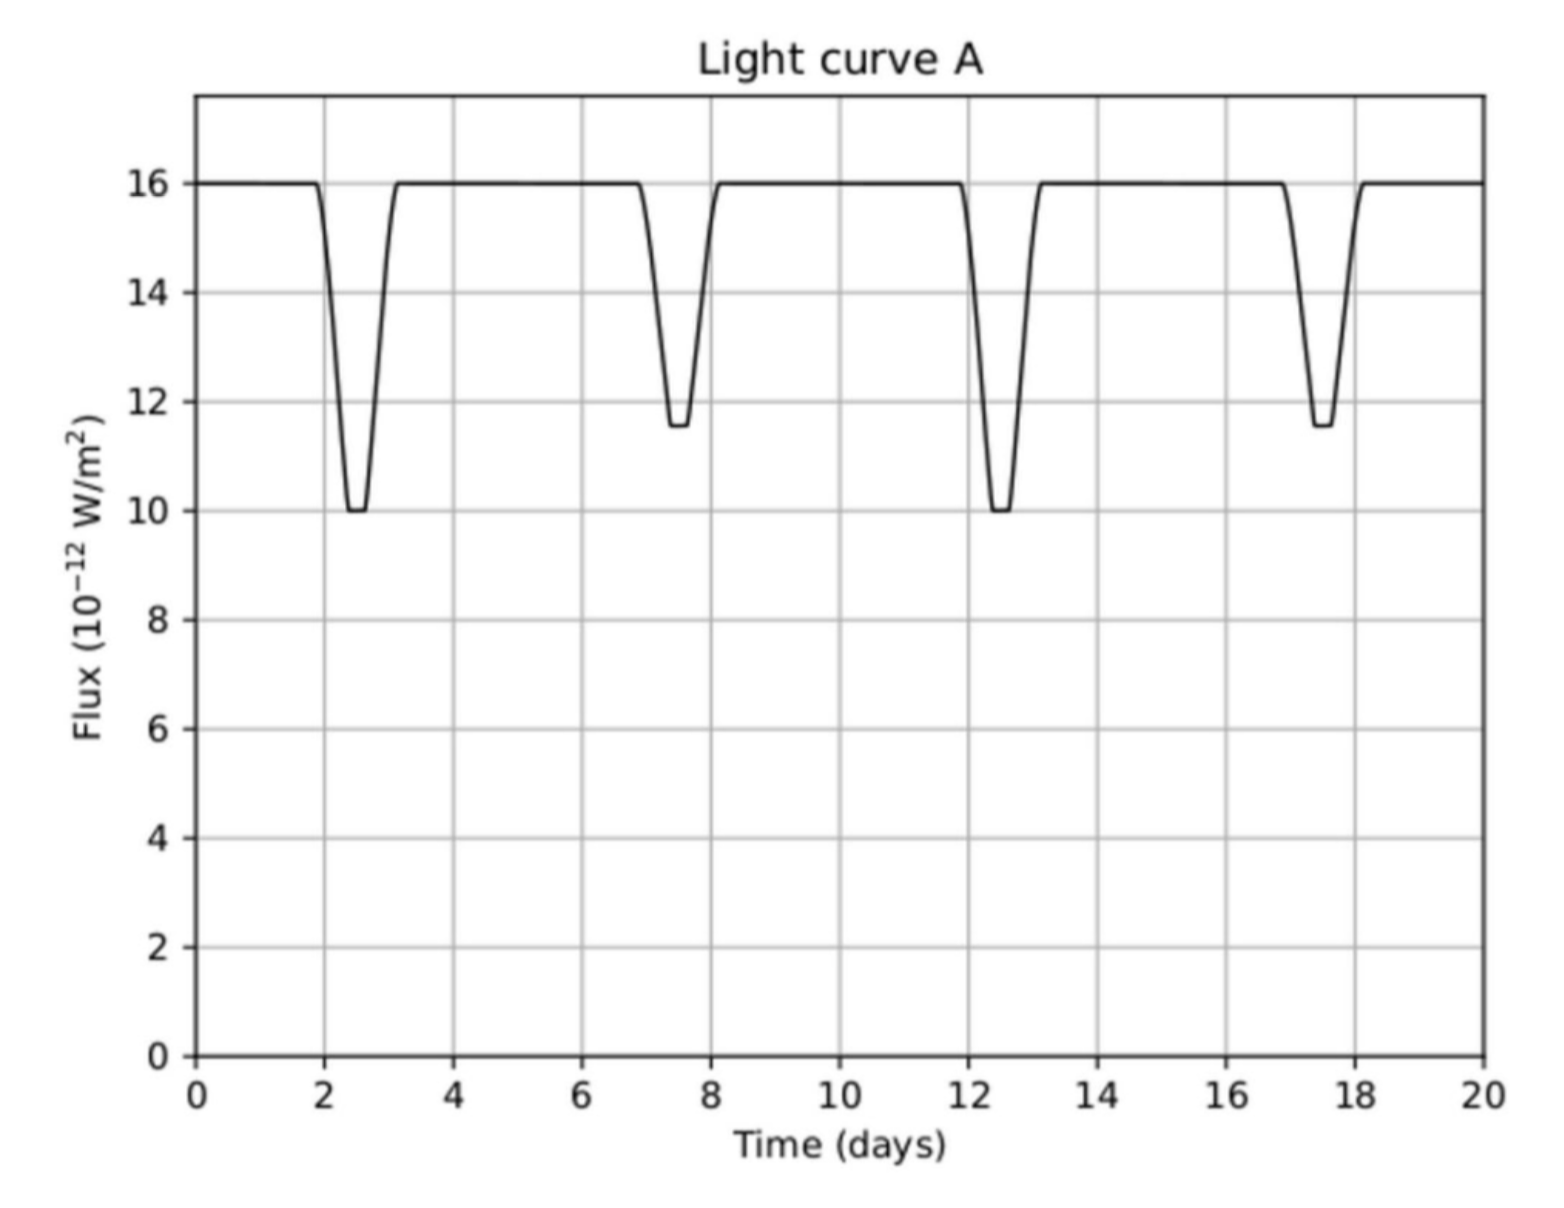
\includegraphics[width = 11cm]{lightcurve}}
	\end{figure}
    
    \begin{enumerate}
        \item Какая из двух звёзд лежит на главной последо- вательности? Выберите более
        вероятный вариант: X или Y .
        \item Определите:
        \item \begin{enumerate}
            \item период системы;
            \item звездную величину каждой компоненты;
            \item отношение радиусов, температур и светимостей звезд.
        \end{enumerate}
    \end{enumerate}
    
    \item Определите суммарную звездную величину скопления содержащего звезды $1^{m}$, $1.2^{m}$, $1.4^{m}$, $1.6^{m}$ и т.д.
    \item Согласно древней средневолжской легенде, в далёком прошлом на небе существовало созвездие Белого Барса (Pardus Album), число звёзд в котором было в точности равно числу букв греческого алфавита, и звёзды эти имели величины $\alpha$ PaA -- $0.10^m$, $\beta$ PaA -- $0.20^m$, $\gamma$ PaA -- $0.30^m$, $\delta$ PaA -- $0.40^m$ и так далее с увеличением на $0.10^m$ вплоть до $\omega$ PaA. Вычислите суммарную звёздную величину звёзд этого созвездия.
    \item Рассчитайте звездную величину звезды, от которой на каждый квадратный метр поверхности Земли приходит около $1000$ фотонов за час.
    \item Известно, что когда Вега находится в зените, от нее на каждый квадратный сантиметр поверхности Земли приходит около $10^6$ фотонов за секунду. Оцените, сколько фотонов за одну секунду приходит на главное зеркало космического телескопа им. Хаббла (HST) от объекта с видимой звездной величинй $30^m$. Диаметр главного зеркала HST составляет $2.4$ метра.
    \item На Земле появился человек с исключительно острым зрением. Чтобы заметить звезду на небе, ему достаточно зафиксировать каждым глазом в среднем по одному фотону от звезды за такт фиксации изображения ($0.04$ секунды). Диаметр зрачка глаза при этом равен $8$ мм, спектральные свойства зрения такие же, как у обычного человека. Какой будет проницающая способность зрения такого человека в звездных величинах? Условия для наблюдений идеальные, атмосферные эффекты не учитывать.
    \item Видимая звездная величина Сириуса  $-1.46^m$. Расстояние до нее составляет $2.64$ пк. Определите абсолютную звездную величину самой яркой звезды на земном небе.
    \item Вычислите абсолютную звёздную величину Антареса, если его параллакс $\pi = 0.0059''$, а видимая звёздная величина $m = 0.91^{m}$.
    \item В некотором созвездии расстояние между звёздами Альфа и Бета на небесной сфере составляет $18^{\circ}$, а их звёздные величины равны $2.96^m$ и $3.07^m$ соответственно. Известно, что абсолютные звёздные величины этих звёзд одинаковы. Какую звёздную величину будет иметь звезда Альфа, если смотреть на неё из окрестностей звезды Бета?
    \item Рассчитайте суммарный блеск $100$ одинаковых звезд с абсолютной звездной величиной $M=5^m$, первая из которых находится на расстоянии $1$ пк, а каждая следующая в $1.2$ раза дальше предыдущей.
    \item Астроном наблюдает два объекта на угловом удалении друг от друга $\alpha=10'$ . Параллакс первого объекта $0.7''$, а параллакс второго объекта $140$~миллисекунд дуги. Один из объектов виден на пределе возможности невооруженного глаза. Определите видимую звездную величину этого объекта при наблюдении со второго. Межзвездным поглощением пренебречь. 
    \item Мы находимся в центре плотного шарового звездного скопления, имеющего радиус $30$~пк. Во сколько раз больше звезд на всем небе видно в телескоп с проницающей способностью $15^m$, нежели невооруженным глазом? Считайте, что звезды скопления похожи на Солнце и равномерно распределены внутри скопления. Влиянием фона неба пренебречь. 
    \item В справочных данных про одно из самых ярких шаровых скоплений NGC $104$ или же Tuc $47$ сказано следующее: «Центральная часть (ядро) шарового звездного скопления имеет светимость равную $10^{4.88}~L_{\odot}$ на кубический парсек и угловой радиус центральной части скопления $0.36'$.»
    Определите видимую звездную величину ядра шарового скопления, если расстояние до него $r_0=4.5$~кпк.
    Межзвездным поглощением пренебречь.
\end{enumerate}
\end{document}